\capitulo{5}{Aspectos relevantes del desarrollo del proyecto}

Lo más relevante de este proyecto es el transformar la última versión de Thoth a una aplicación web hecha por medio de GWT lo que supone comprender el funcionamiento interno del Thoth original, <<desglosándolo>> para poder adaptarlo a las condiciones de un proyecto hecho con GWT.
Estas condiciones limitan un poco la aplicación y nos obligan a reformar partes que antes eran más sencillas.

Además de condicionar Thoth a GWT, también hemos añadido nuevas funcionalidades de las que hablaremos y que completan la aplicación.



\section{Internacionalización}
La aplicación cuenta con la funcionalidad de la internacionalización. Dentro del menú se pueden elegir entre varios idiomas a los que se traducirán los diferentes elementos. Los idiomas en los que está disponible la versión web de Thoth son: Alemán, castellano o español, francés y por supuesto inglés. Consideramos que esta funcionalidad es muy importante para poder llegar a diferentes países en el caso de que fuera necesario.

La internacionalización de la aplicación es un poco diferente a la utilizada en la versión de escritorio de Thoth. En primer lugar es necesario incluir una interfaz con los métodos para la internacionalización y los mensajes <<por defecto>> asociados a cada uno. Cada vez que queramos hacer uso de esos mensajes hay que hacer una llamada al método de la interfaz. Esa interfaz se encuentra en el directorio <<client.gui.utils>> donde se encuentran también los ficheros <<properties>> asociados, donde se encuentran las diferentes traducciones según el mensaje. Estos mensajes son los mismos que los utilizados para la internacionalización de Thoth V2.

Para poder realizar el cambio de idioma es necesario hacer uso de las propiedades las clases <<xml>> y <<html>> de GWT, en concreto <<locale>> que es la que especificará la localidad, que determina el idioma. Por ello cada vez que elegimos un idioma, la aplicación se redirige a una nueva <<URL>> (llevando a cabo una nueva compilación) con el atributo \texttt{locale=} seguido de las siglas del idioma al que se quiere traducir.



\section{Cifrado de contraseñas y seguridad en Thoth Web}

El cifrado de la contraseña es una de las cuestiones más importantes para preservar la seguridad o intimidad del usuario. El porqué es muy simple. Los usuarios normalmente utilizamos las mismas contraseñas o parecidas para cualquier cuenta de una página o red social. Por lo tanto si hay alguien con acceso a la base de datos, podrá ver la contraseña utilizada por un determinado usuario poniendo en peligro esa intimidad no solo en este programa, sino, como ya se ha comentado antes, la de otras cuentas.

Para evitar esto, el método más simple es el cifrar las contraseñas en la base de datos para que en el caso en el que alguien acceda a ella, en el campo <<contraseña>> no vea la contraseña real, sino el resultado del cifrado de esta. El método de cifrado que se emplea en Thoth Web el del algoritmo <<hash>> que como veremos más adelante tiene unas características determinadas. 

\subsection{Funcionamiento del algoritmo hash}

Se trata de un algoritmo matemático con el que se transforma cualquier cantidad de datos en una serie de datos fija que funciona como una huella dactilar. Esto quiere decir que sea cual sea la cantidad de caracteres de entrada, la salida siempre será fija. Cumple además con dos premisas muy importantes para la seguridad: 

\begin{itemize}
\item No es reversible, no se puede descifrar por medio de funciones matemáticas y obtener el resultado antes de ser encriptado, sea cual sea la función utilizada (SHA-1, SHA-2 o MD 5 entre otras, como veremos a continuación).
\item Cuenta con la propiedad de que si la entrada cambia, aunque sea sólo en un bit, el hash resultante será completamente, como se puede ver en la siguiente ilustración \ref{fig:3.1}. En la imagen se puede apreciar que aunque la entrada tenga un mayor numero de caracteres, la salida siempre será de 40 caracteres.

\end{itemize} 

\begin{figure}[h]
\centering
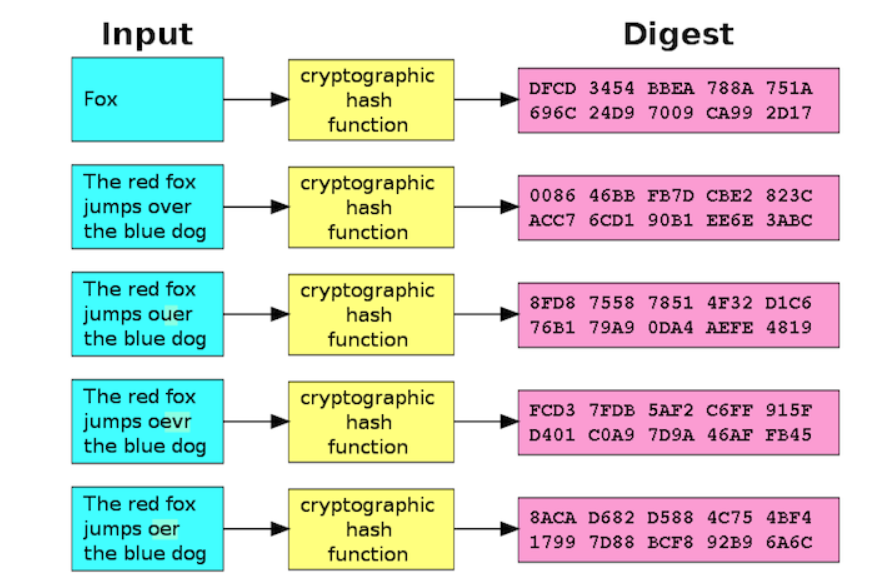
\includegraphics[width=0.99\textwidth]{funcion-hash}
\caption{Aplicación de la función hash a diferentes datos introducidos. \url{https://blog.kaspersky.com.mx/que-es-un-hash-y-como-funciona/2806/}}
\label{fig:3.1}
\end{figure}

Ahora bien, las acciones llevadas a cabo para preservar esa seguridad serían las siguientes: un usuario crea una cuenta en la aplicación, la contraseña se encripta y se almacena en la base de datos. Cuando el usuario trata de iniciar sesión y escribe la contraseña, esta se encripta y se compara el resultado con aquel que se ha guardado en la base de datos, si son iguales el usuario tendrá acceso sino, se le requerirá que lo vuelva a intentar.

El problema principal de esto es que con los avances en temas de seguridad siempre hay asociados otros que tratan de <<romper>> esa seguridad y en este caso no iba a ser menos. Creo que es importante reconocer los peligros que hay asociados a aplicar este método, pero no deseo extenderme demasiado en este aspecto así que los mencionare brevemente.


\begin{itemize}
\item Ataques de fuerza bruta. Consisten en utilizar diccionarios de palabras con contraseñas habituales e introducirlas hasta que alguna coincida. Se trata del ataque menos eficiente, pero el más difícil de evitar.
\item Tablas de búsqueda. Este tipo de ataque si que supondría un grave problema para la seguridad en el cifrado con algoritmo hash. Recordemos que las funciones hash solo se pueden encriptar, no descifrar. Lo que hace este ataque es lo siguiente, cuenta con una tabla de contraseñas típicas y su cifrado hash y las compara con los hash introducidos. Para entender mejor este concepto hay incluso herramientas online que pueden hacer este trabajo. Ver ilustración\ref{fig:3.2}. También las hay que funcionan al revés. Introduces la contraseña que crees que puede usar alguien, la encripta, la compara con todas las de la base de datos y te dice si alguien la utiliza o no.
\end{itemize}

\begin{figure}[h]
\centering
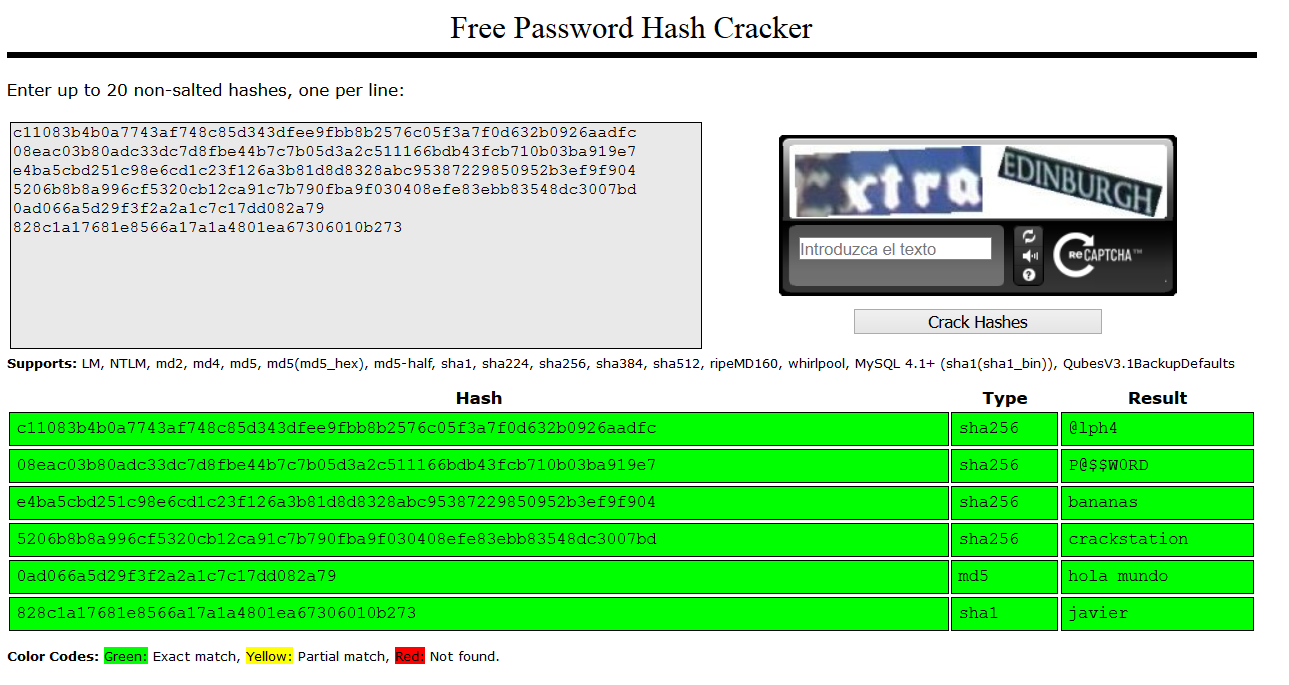
\includegraphics[width=0.99\textwidth]{hash-cracker}
\caption{Ejemplo de ataque con tablas de búsqueda. Imagen sacada de \url{https://crackstation.net/}}
\label{fig:3.2}
\end{figure}

Además de estos, hay más métodos, casi todos basados en las tablas de búsqueda. Según estos ataques queda comprobado que la seguridad de este algoritmo depende en gran mediada de la contraseña que utilice el usuario. Cuanto más aleatoria y con más mezcla de caracteres mejor, ya que formará palabras que no se encuentran en los diccionarios o tablas y solo se podrá descubrir por medio de la fuerza bruta. Entonces ¿cómo hacer que las contraseñas sean más resistentes y solucionar este problema?

Se conoce como el cifrado hash con sal o semilla. Consiste en añadir un conjunto de caracteres aleatorios, agregarlos a la contraseña y una vez hecho esto, cifrarlo con la función hash. De esta manera se consigue que la contraseña sea mucho más aleatoria que la que inicialmente ha introducido el usuario. Así podemos ver como quedaría un intento de <<tablas de búsqueda>> con este tipo de cifrado usa para contraseñas muy simples \ref{fig:3.3}. 

\begin{figure}[h]
\centering
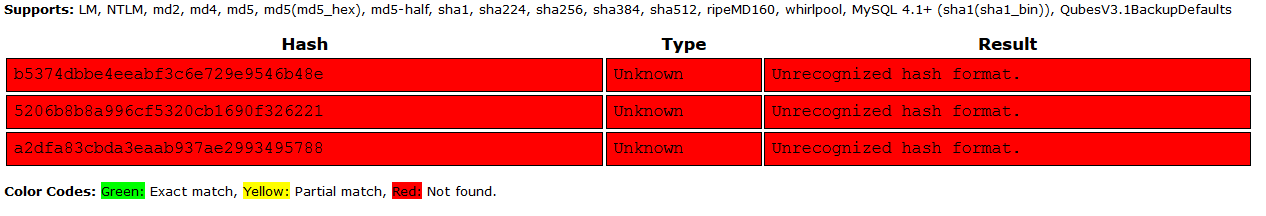
\includegraphics[width=0.99\textwidth]{hash_salt-cracker}
\caption{Resultado de aplicar tablas de búsqueda al cifrado hash con semilla. Imagen sacada de \url{https://crackstation.net/}}
\label{fig:3.3}
\end{figure}

La primera de ellas corresponde con la clave <<123>> la segunda con la palabra <<contraseña>> y la tercera con la fecha <<16-6-17>>. Todas son fáciles, pero al añadirle una clave y cifrarlo todo, se vuelve mucho mas complejo. Se podría pensar que, como la clave que se le añade también se guarda en la base de datos sigue sin ser seguro. Partiendo del hecho de que no hay prácticamente nada seguro al cien por cien, lo que se consigue con esto es dificultar mucho el cálculo, ya que los dos ataques mencionado anteriormente (y varios más basados en estos dos) se ayudan de repositorios de contraseñas. Así si quisieran descifrarlo debería de coger el conjunto aleatorio, sumarle la posible contraseña y cifrarlo comparando los resultados sólo con ese hash (o contraseña cifrada) ya que el salt es único para cada hash. Con este método se consigue que los cálculos para descifrar una contraseña sean bastante más costosos de una forma muy simple.

\section{Google Web toolkit}
Para trabajar con GWT hemos utilizado el entorno de desarrollo de eclipse y ahí 
 
 
 documentar algo del cliente serivido, que me ha costado etc.



\section{Registro e inicio de sesión de usuarios}
Todas las comunicaciones RPC, el porque utilizo modulos de carga, porque dan errores si se encuantran los modulos en las variables a ejecutar el programa.
Sobre la session y la cookies, como utilizo el gwt.xml de app engine y porque da fallo
mensaje de error sin especificar si falla el usuario o contraseña para no mostrar suficiente información como para ponerla en peligro.
